% LaTex Table of Contents, Figures, and Tables example
\documentclass[11pt]{article}
\usepackage{fullpage}
\usepackage{graphicx}
\usepackage{hyperref}


% Header section

\title{CSI 500 Capstone Project}
\author{Jericho McLeod
		\\Department of Computational and Data Sciences
		\\College of Science
		\\George Mason University
		\\Fairfax, VA, USA}


\begin{document}

\maketitle

\begin{abstract}
	
The diffusion of innovation is the study of how, why, and the velocity of the spread of new ideas, products, and innovations a socially dessiminated. This research models the behavior a particular innovative product, the iPad, by identifying the underlying properties that create the most accurate model. Open source languages and tools were used to conduct this analysis, including R, Python, and Netlogo, and the data utilized is iPad sales between 2010 and 2018. The models created were able to approximate the diffusion of innovation for the iPad market with varying degrees of success. This validates prior research in the field, but raises new questions regarding potential model updates.

\end{abstract}


\section{Background}

Innovation takes place via a process whereby a new 'thought, behavior, or thing' is conceived of and brought into reality. No innovation springs full-blown out of nothing; it must have antecedents. Diffusion of innovation occurs along a curve or statistical distribution where the initial participants are the most socially influential in the diffusion of innovation. This can be more valuable than traditional advertising, a fact that the marketing industry has noted and now is academically included in relevant curriculum. This is evident in the current market selection of social influencers, and can be tracked through new product releases through such individuals in social media: this agrees with the final point of the article, in that it shows the history of concerns expressed being mitigated by marketing innovators through specific action  \cite{Robertson67}.


Diffusion studies rely on the study of change in behavior rather than an observation at a fixed time, offering advantages over other types of research. However, focus had been lost on the value of innovations during the 1970s, as well as focus on well-conducted scientific study, seeing the rise of the misuse or ignoring of such factors as causality, unitary measurement, and other cognitive biases. The author noted that this was being overcome at the time by reapplying social structure in diffusion research via such methods as network analysis \cite{Rogers76}.


This paper examines the diffusion of Apple's iPad utilizing several models with and without the inclusion of a social network. The iPad product line has spanned nearly a decade, and several new varieties have been created. Several models will be created and evaluated on how well they can be fitted to the observed market behavior of the iPad product famiily. From this, inferences will be made regarding the importance of social networks on this particular innovation, as well as whether it remains appropriate to label the product family a single innovation. 


\section{Methods}

\subsection{Python Methods}

A Python model was constructed to illustrate the Diffusion of Innovation of the iPad. The behaviors being simulated were adoption and disposal of an innovation. In order to do simulate these behaviors a series of Python classes were created to represent individuals, classes of individuals within a population, and the diffusion model. The first class created was the Person class. This contained a status for instantiated Person objects along with function definitions to update statuses.


Next, the Population class was created. This class contained the population features for adoption and disposal rates and contained a group of Person objects in three compartments based on the Person object's current status. This class also contained the triggers for moving a Person object to the subsequent status in the model based on comparing the adoption and disposal rates, Beta and Gamma, to randomly generated numbers. 


The final class was the model itself. The model instantiates a population with defined parameters, then iterates through updates to shift the population through the process of adopting and disposing of an innovation a set number of times. Finally, the model class creates a visualization of the resulting curves.

\subsection{R Methods}

A matrix model of the Diffusion of Innovation was also constructed using the R language. This model was much more simple in its construction: it contained variables for the populations of the three categorical stages of Diffusion of Innovation, along with probabilities for moving from the initial category of Potential to the Adopters category and from the Adopters category to the Disposers category. The quantities at each iteration, representative of a month in real time, were saved, allowing for subsequent review of the model's results. The same variables, Beta and Gamma, from the Python model were used in the R model, albeit with different values.


The beta and gamma constants are defined first in this model, and represent that adoption and disposal rates of the population for the studied innovation. This is followed by a matrix of the probability of membership in a class given current membership in a class, to be used in running the model to calculate movement between classes. The classes were then assigned starting populations as variables, and a vector of the current class participation was created. An output print function was created, followed by a vector for each class to store values across the simulation. Then the time range variable was instantiated as a sequence of specified length.


The model itself consisted of multiplying the vector of current population percentages with the matrix of probabilities of shifting classes. This was performed iteratively to the limit of time specified previously, with results being stored in the created vector. The results were then plotted to allow interpretation of the results and tuning of the model to match observed market data.


\subsection{NetLogo Methods}

The NetLogo model simulated the addition of a social network to the parameters of prior models. This was done via addition of edges representing social connection between nodes representing individuals. The edges were distributed by first assigning each node a quantity of originating edges from a poisson distribution, then finding partners for each outgoing edge at random. Then, adoption and disposal were undertaken only when a sufficient quantity of a node's neighbors had reached this stage; these quantities were beta and gamma in the model. 


\subsection{Data}
As an example of the Diffusion of Innovation, one can consider the sales of consumer electronics. For this study, the data to be examined will be that of sales data for the iPad. The iPad was the first widespread consumer tablet, and as such, represented an innovation. Being a product of a company that is publicly traded in the United States of America further means that sales data are easily obtained, making it a good candidate for study. Plotting the sales data for the iPad reveal an easily discernable curve (see figure \ref{fig:iPad_adoption}).

\begin{figure}[h!]
	\centering
	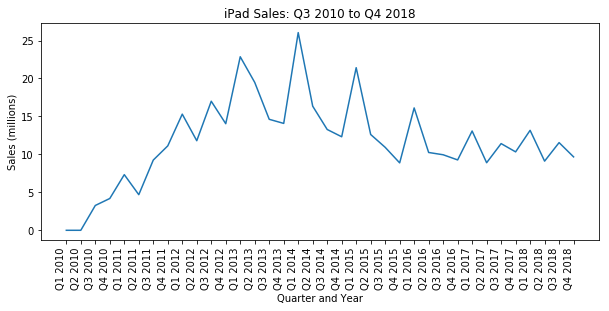
\includegraphics[width=0.7\linewidth]{Diffusion_ipad.png}
	\caption{iPad Sales}
	\label{fig:iPad_adoption}
\end{figure}


\section{Results}

\subsection{Python Model}

Population size parameters of the model primarily impact the smoothness of the resulting curves and the time it takes to run the model, with the two values being highly correlated in that increasing the smoothness of the output takes more time to run.

Beta, as the adoption rate in the model, impacts the speed at which the population moves between categories. Thus, at Beta = 1, all adoption happens in iteration 1, and at Beta = 0.0001, the adoption rate is extended in time, and approaches infinity as Beta approaches 0. Gamma, the disposal rate of the model, performs identically to beta with the exception of the fact that Gamma is subsequent to, and thus dependent on, Beta.

Time periods do not effect the behavior of the model directly, merely the amount of observation of the model that is conducted. If a model appears to be merely a set of straight lines or very steep curves, altering the time period may be helpful in understanding the input beta and gamma.

By adjusting these values until a satisfactory output was created, an approximation of the Diffusion of Innovation for the iPad was created. The Population size used was N=10,000, and the number of iterations was 1,000. Beta and Gamma were, respectively, 0.003 and 0.008. The results of this curve can be seen below in figure \ref{fig:Diffusion_graph}.

\begin{figure}[h!]
	\centering
	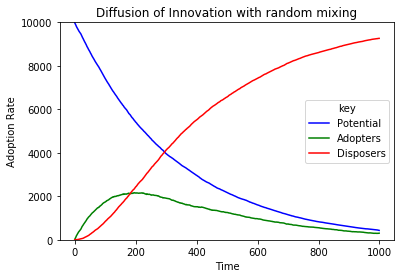
\includegraphics[width=0.7\linewidth]{Diffusion_graph.png}
	\caption{Python Diffusion of Innovation Model: iPad}
	\label{fig:Diffusion_graph}
\end{figure}


\subsection{R Model}

When running the Diffusion Model using Matrix methods in R, population size was not adjusted, as the R plotting method returns smooth results even with small populations. The time period over which the model was run was limited to the periodicity in the market data to more closely match the observed behavior. While this limits comparability of the two models' beta and gamma, the relationship between them may still be meaningful. 

In this model, the beta and gamma that most closely matched observed behaviors was 0.08 and 0.25. In both cases, the gamma value is nearly three times higher than the beta value, indicating a much faster disposal rate than adoption rate, albeit from a generally smaller population size. The observed model performance can be reviewed in figure  \ref{fig:Diffusion_graph_2} below.

\begin{figure}[h!]
	\centering
	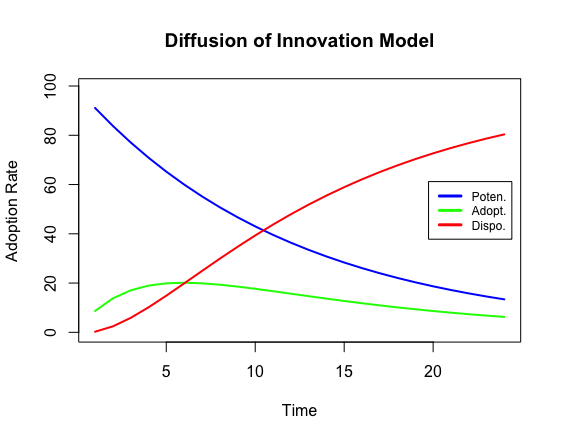
\includegraphics[width=0.7\linewidth]{Rplot02.png}
	\caption{R Diffusion of Innovation Model: iPad}
	\label{fig:Diffusion_graph_2}
\end{figure}



\subsection{NetLogo Model}

This model is unique compared to the others in that unchanged parameters can yield highly varied stable states. For some sets of parameters, a network can end in a state of having never adopted an innovation, a state of complete adoption, or a state of complete disposal. It is more common, however, to reach a stable state with some mixture of these. Prior models always resolved to a state of having moved all individuals from potential to adopter, then from adopter to disposer. Including a social network causes the final state to more closely resemble observable behavior. As one can see in figure \ref{fig:Diffusion_NetLogo}, a similar adoption curve can be seen in the 'Population Types' plot to that of the sales rate of iPads, while retaining some portion of the population in the potential category. This represents the individuals who never adopted the technology in part due to never receiving the social influence from peers to do so, as shown in blue in the network. 

However, comparing this model to prior models reveals a shortcoming in that adoption and disposal rates tended to be more symmetrical due to being a more compressed model parametrically speaking. Beta and Gamma parameters needed to be near narrow bands based on the network density in order for the model to show any evolution. 
\begin{figure}[h!]
	\centering
	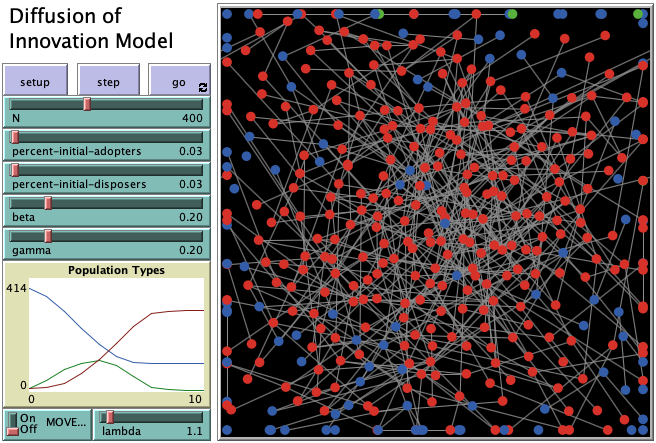
\includegraphics[width=0.7\linewidth]{Diffusion_NetLogo.png}
	\caption{NetLogo Diffusion of Innovation Model: iPad}
	\label{fig:Diffusion_NetLogo}
\end{figure}

\subsection{Model Comparison}
The three models created vary in applicability for differing modeling purposes. The NetLogo model offers what may be considered the most realistic model based on the inclusion of a social network, but requires additional parameter tuning in order to more reliably replicate observed behaviors. Conversely, the R model offers an advantage in simpliciity, and would be the most likely candidate for exploratory analysis of a system. The Python model offers increased flexibility over the R model through the creation of classes, but less realistic results than the NetLogo model. 




\section{Discussion}

In the observed data from Quarter 1, 2010, to Quarter 4, 2018, iPad sales appear to reach a point of peak adoption, followed by a slow decline, and end with a period of relatively level sales. In the initial models, where the total number of adopters provided the pool from which disposers were created, there are not enough parameters to recreate this trend entirely. Utilizing a low beta, or slow adoption rate, followed by a higher gamma, or faster disposal rate, a relatively steep growth period could be shown that would then be minimized by the faster disposal rate, approximating the level of sales late the iPad lifecycle. This falls short of matching the visually apparent derivative of the moving average of the sales data. The NetLogo model is unable to replicate this entirely. In social networks, much higher disposal rates for an innovation lead to rapidly stifled growth. 

\section{Conclusions}

The shortcomings of the models highlights the possibility of additional components that have not yet been identified and included. One such component could be original innovations occurring within the product famiily that are being captured in aggregated sales data. An second additional component may be shifts in consumer opinions; individuals are not limited by previous decisions. A third such component is shifting social networks. 

\section{Future Research}

The combination of these three potential updates to existing diffusion models may yield better results in terms of explaining the diffusion of iPads through a population. Future research with the addition of additional sales data, segregated by individual product lines within the product family, alongside additional parameters to regress through the innovation pipeline and dynamic social networks, is needed to answer these questions.


\bibliographystyle{plain}
\bibliography{Final_paper_bib}

\end{document}